% Auto-generated editable source. Edit freely in VS Code.
% Parallel source; the live site is pages/proj-benchmark-selection.html.
\documentclass[11pt]{article}
\usepackage[margin=1in]{geometry}
\usepackage{graphicx}
\usepackage{hyperref}
\usepackage{xcolor}
\definecolor{aidred}{HTML}{A8324A}
\definecolor{aidpink}{HTML}{CF4D87}
\hypersetup{colorlinks=true,linkcolor=aidpink,urlcolor=aidpink,citecolor=aidpink}
\newcommand{\finding}[2]{\par\medskip\noindent{\color{aidred}\textbf{Finding #1.}}~#2\par\medskip}

\title{Does Benchmark Correlation Predict Selection Quality?}
\author{Saanvi S. Subramanian \\ \small California Institute of Technology}
\date{\small Trust-AI-Eval and GEM-Bio @ NeurIPS 2026 \quad\textbullet\quad sole author}
\begin{document}
\maketitle

\begin{abstract}
\noindent A protein benchmark reports the Spearman correlation between model scores and measured outcomes, which summarizes ranking quality over a whole assay. A design campaign does something else: it takes the top few candidates and tests them. Those are different quantities, and this measures how much the first predicts the second, across 70 benchmark units in four corpora: 41 ProteinGym scans, 16 SSMuLA combinatorial libraries, three Rubisco kinetic axes from 8{,}760 single mutants, and 10 PETML plastic-degradation campaigns. Reported correlation explains half the variance in top-10\% selection value and 16\% at top-1\%, the same correlation delivers different selection value in different benchmark families, and a label-free skew diagnostic that looks promising reverses sign across corpora. Where a supervised model has genuine signal the two improve together, so the claim is scoped, not blanket.
\end{abstract}

\section*{Correlation stops predicting where campaigns act}

\finding{1}{Correlation becomes less informative exactly where campaigns act. It explains half the variance in top-10\% selection value and 16\% at top-1\%. Three of the 41 ProteinGym assays produce worse-than-random top-1\% selections despite positive reported correlations, the worst at selection value $-0.300$ on a reported $\rho$ of $+0.105$.}

\begin{figure}[h]\centering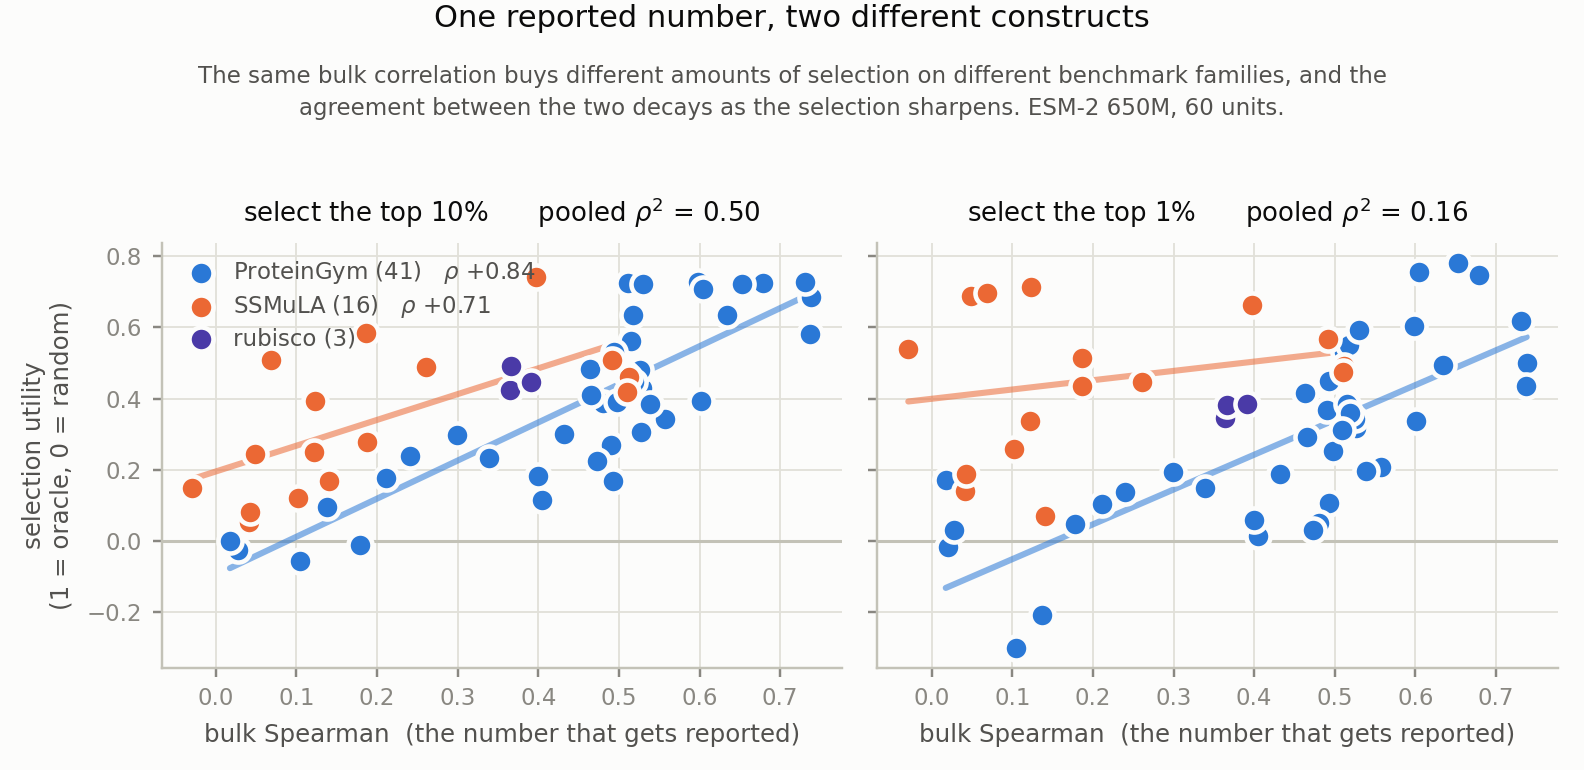
\includegraphics[width=\textwidth]{../../assets/images/projects/agentevals/selection-decay.png}
\caption*{\textcolor{aidred}{\textbf{Figure 1. Reported correlation against selection value.}} Each point is one benchmark unit. The relationship weakens sharply at the tighter cutoff, and three ProteinGym assays fall below zero at top-1\% despite positive reported correlations. Per-corpus fits have similar slopes but different intercepts, the family offset the next figure tests.}\end{figure}

\finding{2}{The same reported correlation means different things in different benchmark families. At matched correlation, SSMuLA libraries deliver $+0.265$ more top-1\% selection value than ProteinGym assays (Mann-Whitney $p=0.0001$), and $+0.147$ at top-10\% ($p=0.0022$). A second scorer family reproduces the offset at $+0.252$ ($p=0.0003$). An aggregate leaderboard score mixes model behavior with benchmark composition.}

\begin{figure}[h]\centering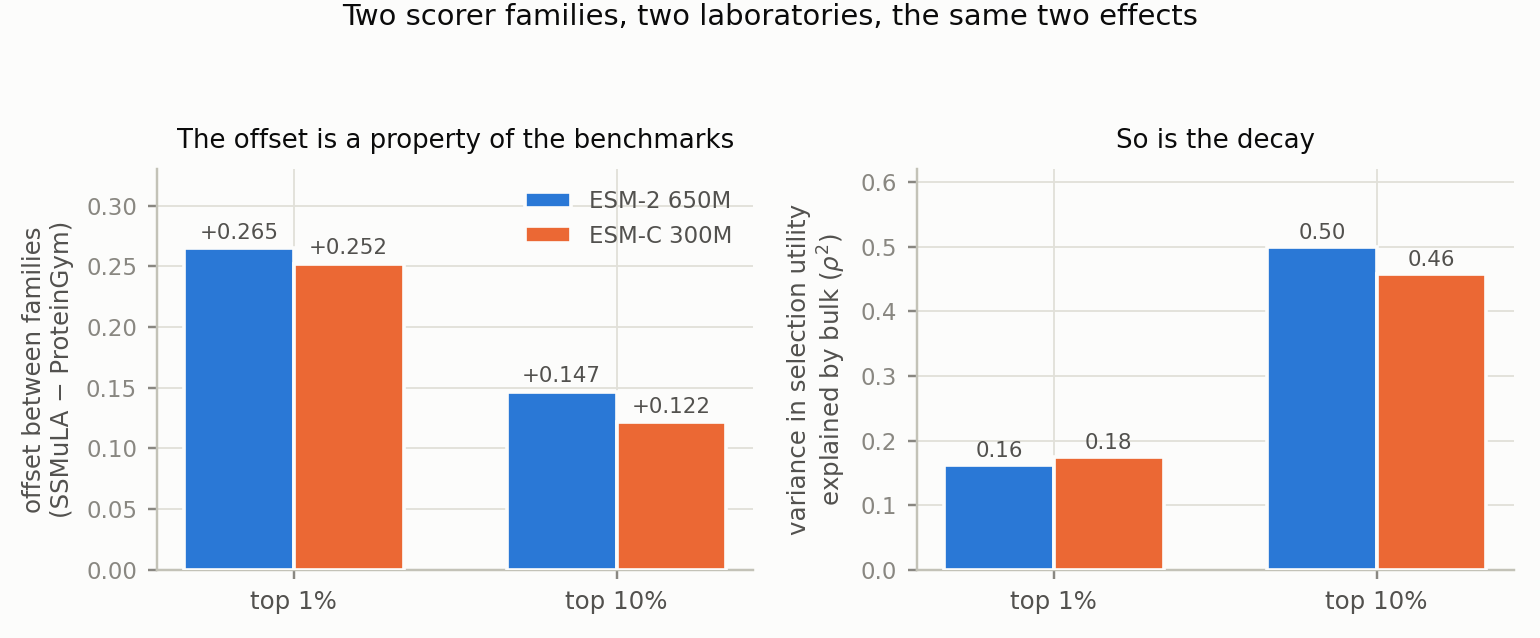
\includegraphics[width=\textwidth]{../../assets/images/projects/agentevals/selection-replicate.png}
\caption*{\textcolor{aidred}{\textbf{Figure 2. The offset replicates under a second scorer.}} Two scorer families from different laboratories agree at the unit level, correlating at $+0.892$ on reported correlation and $+0.899$ on top-1\% selection value, so the offset is a property of the benchmark families rather than of any one model.}\end{figure}

\finding{3}{The obvious label-free fix does not transfer. Score-distribution skew correlates with residual top-1\% selection value at $+0.633$ across 60 units, but its sign reverses across families: fitted on ProteinGym and applied to SSMuLA it gives $-0.388$, and a fourth corpus reverses it again, $-0.783$ within PETML against $+0.551$ within ProteinGym. Skew adds information alongside the reported correlation, and fails as a standalone transferable rule.}

\finding{4}{The critique has a boundary. Where a supervised model has genuine signal, correlation and selection improve together: across 12 assays and three cross-validation schemes on identical folds, mean selection gain is $+0.035$ at both cutoffs against a bulk correlation gain of $+0.031$. The narrower attribution problem survives: per-unit correlation and selection gains track at top-10\% ($\rho=+0.679$) but not at top-1\% ($\rho=+0.168$, $p=0.33$).}

\paragraph{What the GEM-Bio side adds.} A top-20\% cutoff that all four corpora support, where the PETML result lives: selecting the top 20\% of variants on 10 plastic-degradation studies captures essentially none of the achievable gain, $-0.016$ for ESM-2 and $-0.006$ for ESM-C, against $+0.326$, $+0.461$ and $+0.423$ on SSMuLA, Rubisco and ProteinGym. And the Rubisco controls: ESM-2 reaches $\rho=+0.631$ against maximum turnover across 8{,}760 single mutants, restricting to well-measured variants drops it to $+0.364$, and partialling out wild-type residue preference drops it to $+0.259$.

\begin{figure}[h]\centering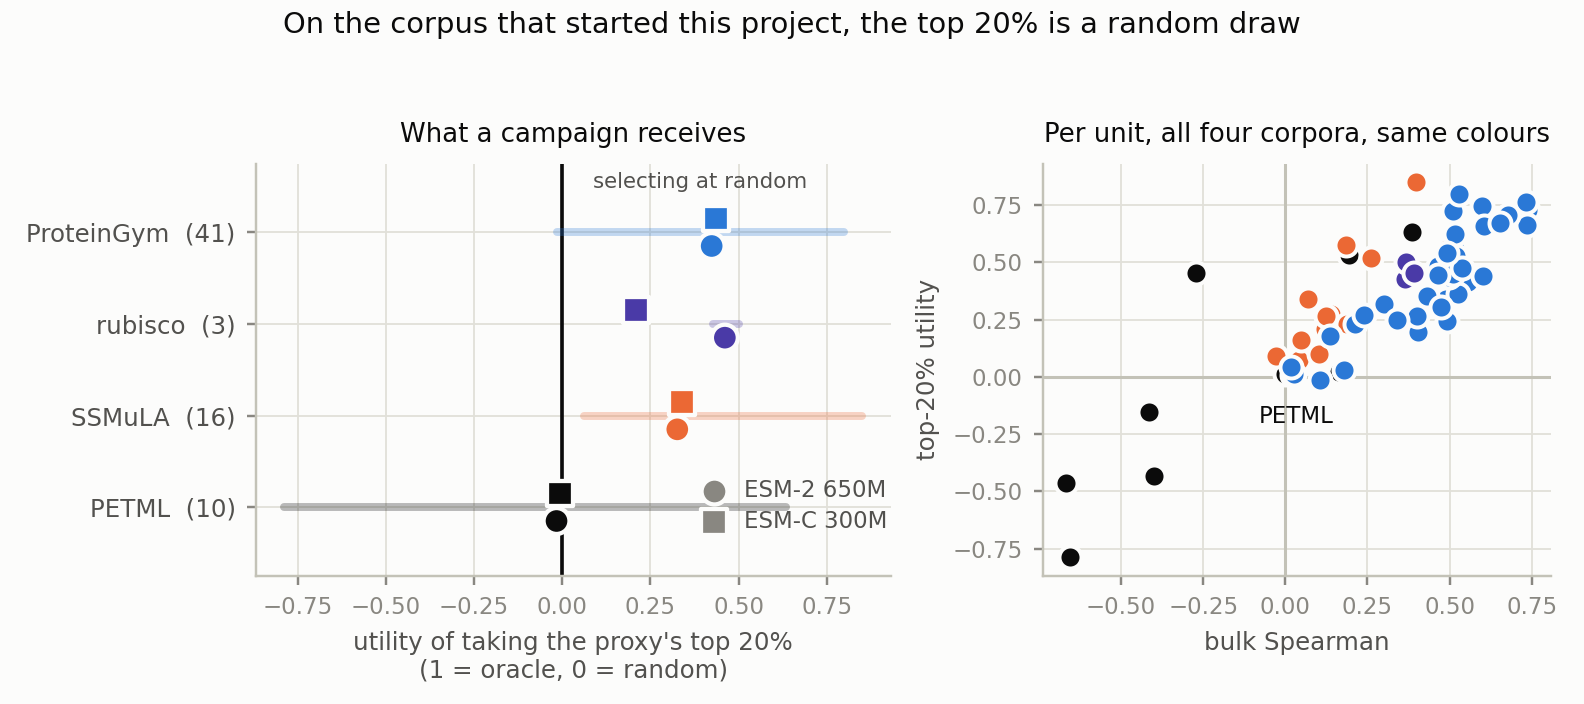
\includegraphics[width=\textwidth]{../../assets/images/projects/agentevals/selection-campaign.png}
\caption*{\textcolor{aidred}{\textbf{Figure 3. Selection utility at the cutoff all four corpora support.}} Left, mean top-20\% selection utility per corpus under both model families; right, all 70 units separately. The plastic-degradation studies sit near zero while the other three corpora are clearly positive. The power analysis puts 10 studies far below what a precise between-corpus comparison would need.}\end{figure}

\section*{Limitations}
One scientific domain, and units within a corpus share experimental conventions, so they are not fully independent. The family offset is estimated from ProteinGym and SSMuLA only; Rubisco and PETML are too few or too heterogeneous to estimate comparable offsets. The mechanism behind the offset is unidentified, and the between-corpus PETML comparison is underpowered at 10 studies.

\end{document}
